\scanpage{18}
% Top-edge pencil note; the final 3.1 is on a second, lower line.
\margin{\handwritten{\unsure{1.93|1.95}, 1.27, 2.9 à reporter au \unsure{n\textsuperscript{o} 3}\unsure{?}\\3.1}}

\(\mathbb{S}\)GA 4 VI

\uline{Sommaire}
\margin{\handwritten{\uline{\unsure{pp|pr}}}}

1. Conditions de finitude pour les objets et flêches d'un topos.\margin{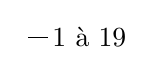
\begin{tikzpicture}[baseline=(r.base),x=0.25cm,y=0.25cm]\node[anchor=west,inner sep=0] (r) at (0,0) {\handwritten{1 à 19}};\draw (-1.2,0)--(-0.2,0);\end{tikzpicture}}

2. Conditions de finitude pour un topos.\margin{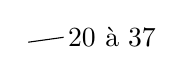
\begin{tikzpicture}[baseline=(r.base),x=0.25cm,y=0.25cm]\node[anchor=west,inner sep=0] (r) at (0,0) {\handwritten{20 à 37}};\draw (-2,-0.25)--(-0.2,0);\end{tikzpicture}}

3. Conditions de finitude pour un morphisme de topos. \deleted{\handwritten{Cas des \illegible{2}}}\margin{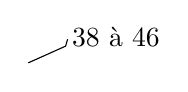
\begin{tikzpicture}[baseline=(r.base),x=0.25cm,y=0.25cm]\node[anchor=west,inner sep=0] (r) at (0,0) {\handwritten{38 à 46}};\draw (-2.2,-1.3)--(-0.3,-0.45)--(-0.2,-0.1);\end{tikzpicture}}

\deleted{4. Constructibilité.}\inserted{\handwritten{4. Conditions de finitude pour un topos \inserted{obtenu par} recollement.}}\margin{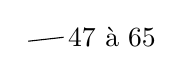
\begin{tikzpicture}[baseline=(r.base),x=0.25cm,y=0.25cm]\node[anchor=west,inner sep=0] (r) at (0,0) {\handwritten{47 à 65}};\draw (-2,-0.2)--(-0.2,0);\end{tikzpicture}}

% Pencil divider after item 4; the relocation arrow terminates here.
\noindent\hspace*{-1cm}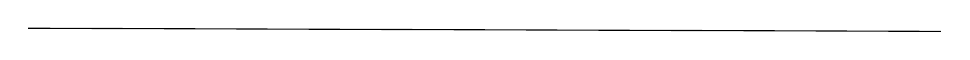
\begin{tikzpicture}[x=0.95cm,y=0.5cm]
\draw (0,0)--(12.2,-0.08);
\end{tikzpicture}
% Left-margin curve, source query, and brace. The lower curve meets the circled 5 below.
\reversemarginpar
\margin{\begin{tikzpicture}[x=0.45cm,y=0.45cm]
\draw[->] (3.6,-7.3) .. controls (-0.3,-4.7) and (-0.1,-3.3) .. (1.5,-1.8) .. controls (2.2,-1.0) and (3.0,-0.4) .. (3.7,0);
\node[anchor=east] at (1.0,-1.9) {\handwritten{\unsure{?}}};
\draw (3.0,-2.9) .. controls (3.0,-3.8) and (3.0,-3.9) .. (2.7,-4.0) .. controls (3.2,-4.1) and (3.2,-4.7) .. (3.0,-5.3) .. controls (2.95,-5.5) and (3.0,-5.6) .. (3.2,-5.7);
\end{tikzpicture}}
\normalmarginpar

\deleted{5}\handwritten{6}. Catégories fibrées et $\underset{\handwritten{\longrightarrow}}{\mathrm{Lim}}$ (rappels).

\deleted{6}\handwritten{7}. Sites et topos fibrés.

\deleted{\unsure{7}}\handwritten{8}. Limites projectives de topos.

\deleted{8}\handwritten{\unsure{8|9}}. Cas des limites projectives filtrantes de topos cohérents par morphismes de transition cohérents: théorèmes de passage à la limite pour la cohomologie.

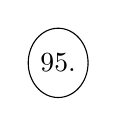
\begin{tikzpicture}[baseline=(n.base)]
\node[inner sep=1.5pt] (n) {\deleted{9}\handwritten{5}.};
\draw (n.center) ellipse [x radius=0.38cm,y radius=0.44cm];
\end{tikzpicture}
Cohomologie d'une limite inductive de fais\unsure{\deleted{c}x|\deleted{x}c}eaux sur un topos cohérent
% The right edge removes any space where final punctuation could have stood; no point is visible.

\reversemarginpar
\margin{
\begin{tikzpicture}[x=0.3cm,y=0.3cm]\fill (0,0)--(0.12,0.6)--(0.34,0.65)--(0.29,0.05)--cycle;\end{tikzpicture}}
\normalmarginpar
\handwritten{10. Appendice (par P. Deligne). \deleted{\unsure{Existence de points} \unsure{d'}}Un topos cohérent a \inserted{\unsure{suffisamment} de points}.}

\deleted{NB Bien sûr \deleted{\unsure{9|8}}\handwritten{8} serait interchangeable avec le bloc \deleted{5}\handwritten{4} à \deleted{8}\handwritten{\unsure{7|9}}. Mais il me semble plus naturel de mettre dans deux numéros consécuti\unsure{\deleted{s}f|\deleted{f}s}s les deux facettes d\unsure{\deleted{g}u|\deleted{u}g} passage à la limite en cohomologie. Bien sûr, le numéro \deleted{\unsure{9|8}}\handwritten{8} sera réduit à une ou deux pages, le sorite des conditions de finitude étant déjà fait.}

\deleted{Le n\textsuperscript{o} 4 contiendra le sorite des groupes constructibles (au sens groupes finis ou non), des faisceaux de torsion, des notions de constructibilité pour les Modules et complexes de Modules, - y compris les faits spéciaux dans le cas localement noethérien. Je pense que je le rédigerai mais ne le garantis pas. On peut \deleted{à la rigue} laisser t\deleted{\unsure{l|i}}\handwritten{o}mber le n\textsuperscript{o}4, ce sera alors moins beau bien sûr ...:}

% The large diagonal cancellation continues through this third typed paragraph.
\deleted{La rédaction qui suit des n\textsuperscript{o}s 1 à 3 est ào\unsure{\deleted{p}m|\deleted{m}p}plète, à cela près que je compte y ajouter encore quelques exemples (en particulier un topos localement algébrique non algébrique\inserted{\handwritten{)}}\unsure{,|.} \deleted{un morphisme non cohérent de topos cohérents).}}
\reversemarginpar
\margin{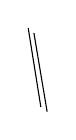
\begin{tikzpicture}[x=0.4cm,y=0.4cm]\draw (0,2.5)--(0.4,0);\draw (0.18,2.35)--(0.6,-0.15);\end{tikzpicture}}
\normalmarginpar
% Doubt around the whole insertion concerns cancellation scope: a long diagonal also crosses its words.
\unsure{\inserted{\handwritten{et un topos ayant une famille génératrice formée d'objet\unsure{s} cohérents, qui n'est pas localement algébrique}}}
% archive sheet number: 17

